\documentclass{article}
\usepackage{pgfplots}
\usepackage{tikz}
\usepgfplotslibrary{fillbetween}
\pgfplotsset{compat=1.18}

\begin{document}

\section*{Test Plot: HHL Circuit Depth}

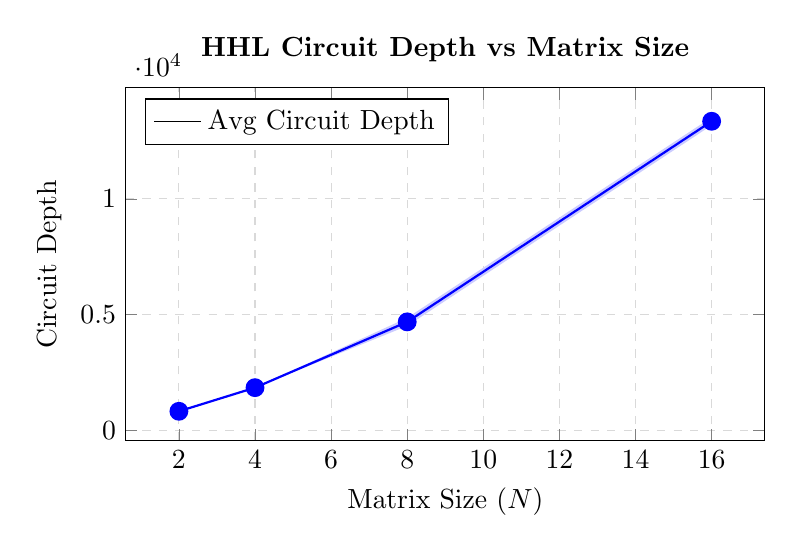
\begin{tikzpicture}
\begin{axis}[
    width=0.8\textwidth,
    height=0.5\textwidth,
    xlabel={Matrix Size ($N$)},
    ylabel={Circuit Depth},
    title={\textbf{HHL Circuit Depth vs Matrix Size}},
    grid=major,
    grid style={dashed, gray!30},
    legend pos=north west,
    mark size=3pt,
]

% Upper bound for error region
\addplot[
    name path=upper,
    draw=none,
] coordinates {
    (2, 817.9)
    (4, 1839.4)
    (8, 4858.5)
    (16, 13527.0)
};

% Lower bound for error region
\addplot[
    name path=lower,
    draw=none,
] coordinates {
    (2, 816.4)
    (4, 1838.8)
    (8, 4507.2)
    (16, 13180.3)
};

% Fill between upper and lower
\addplot[blue!20] fill between[of=upper and lower];

% Main line plot
\addplot[
    blue,
    thick,
    mark=*,
] coordinates {
    (2, 817.1)
    (4, 1839.1)
    (8, 4682.9)
    (16, 13353.6)
};
\addlegendentry{Avg Circuit Depth}

\end{axis}
\end{tikzpicture}

\vspace{1em}

\textbf{Figure 1:} HHL Circuit depth scaling with matrix size. The circuit depth increases significantly as the problem size grows.

\end{document}
